\section{Formation control + motoroplysninger}
%\addbibresource{bib.bib}
\head{This section will give a short introduction to formation control in general followed by some of the individual assignments which needs to be determined before the process of design can be started.}
The theory of formation control in general is widely applied. It can be applied in assignments regarding control of robots which needs to be placed relative to each other. Depending on the given task of the robots, and which type of robots are in focus, the formation can be utilized in different ways. The robots can also be of various types: Swarm robots, driving vehicles, helicopters, aeroplanes, ships etc. which can both be manned and unmanned. The tasks that these robots needs to fulfill can vary a lot and be both as individuals in a formation or as a whole group. Swarm robots in general got many purposes such as vacuum cleaning robots, who needs to clean a rather large area or flying robots like quadcoptors who can make different kinds of assignments. When these quadcoptors work as a combined group they could lift a certain amount of payload to achieve their goal as a group, or they could work individually in a network to do several smaller tasks. An example of how quadcoptors are working together can be examined at \citep{ethswarm}.

Within the scope of this project the robots will be unmanned ships, \ac{ASV}. The ship's main purpose will be to map the sea bed by using sonars. When one ship need to do this alone, and due to the range of the sonar, the time spend could be improved. The sonar scanning would be done as seen on figure \missingfigure{Billede af enkelt baad som anvender sonar til at scanne havbund}. When only one ship need to map a complete sea bed this process could take up a lot of time dependent on the area that need to be covered. The time spend could be improved to make this mapping more efficient. One way of optimizing the time used is to add more ships to help map the sea bed. To make the process of this as optimal as possible it could be of benefit to implement formation control in the specific assignment. This could be done in several ways, but is mostly thought of in a rigid formation, such that the formation maps the same area of the sea bed the whole time. The idea can be seen on figure \missingfigure{Billede af flere baade som anvender sonar til at scanne havbunden}. The distances between the ships would be determined by how far the sonars could reach the sea bed. There should be some overlap of the maps from each sonar but still as little as possible. The specific formation could be a simple line or it could be more advanced formations. This does not have any relevant impact of how the mappings of the sea bed would be due to the subsequent processing of the collected data from the maps. Different formations of ships can be seen on figure \ref{fig:diffforms}.
\begin{figure}[ht]
	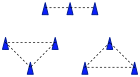
\includegraphics[width=0.5\textwidth]{fig/diffforms}
	\caption{Different formations which the \ac{ASV}s can make.}
	\label{fig:diffforms}
\end{figure}
The formation 


\textbf{inline 475:}\\
g6606\\
58 euro\\
1217 kv\\
aksel 3.17mm\\
nom 11.1V max 14.8V\\

\textbf{compact 460z:}\\
g7741\\
46 euro\\
900 kv\\
aksel 4mm\\
nom 14.8V max 18.5V\\

\textbf{compact 465z:}\\
7772\\
64 euro\\
600 kv\\
aksel 5mm\\
nom 14.8V max 18.5V\\
